\section{Optik}

\subsection{Brechung}

\begin{boxleft}\bla{Brechung}
\des{n_1}{Brechzahl Medium 1}\\
\des{n_2}{Brechzahl Medium 2}\\
\des[\radian]{\varepsilon_1}{Einfallwinkel (Medium 1)}\\
\des[\radian]{\varepsilon_2}{Ausfallwinkel (Medium 2)}\\
\des[\meter\per\second]{c_1}{Phasengeschwindigkeit (Medium 1)}\\
\des[\meter\per\second]{c_2}{Phasengeschwindigkeit (Medium 2)}
\end{boxleft}\begin{boxrightshaded}
\begin{align*}
\frac{\sin{\varepsilon_1}}{\sin{\varepsilon_2}}&=\frac{n_2}{n_1}=\frac{c_1}{c_2}\\
\varepsilon_2&=\arcsin{\frac{\sin{\varepsilon_1}\cdot n_1}{n_2}}
\end{align*}
\end{boxrightshaded}

\begin{boxshaded}
\begin{align*}
&\text{Totalreflexion tritt nur auf wenn der Lichtstrahl von einen dichteren in ein wenniger dichten Stoff übergeht}
\end{align*}
\end{boxshaded}

\begin{boxleft}\bla{Totalreflexion}
\des{n_1}{Brechzahl Medium 1}\\
\des{n_2}{Brechzahl Medium 2}\\
\des[\radian]{\varepsilon_g}{Einfallwinkel (Medium 1)}
\end{boxleft}\begin{boxrightshaded}
\begin{align*}
\sin{\varepsilon_g}&=\frac{n_2}{n_1}
\end{align*}
\end{boxrightshaded}


\subsection{Hohlspiegel}

\begin{boxleft}\bla{Spiegel}
\des[\metre]{f'}{Brennpunkt}\\
\des[\metre]{a'}{Bildweite}\\
\des[\metre]{y'}{Bildgröße}\\
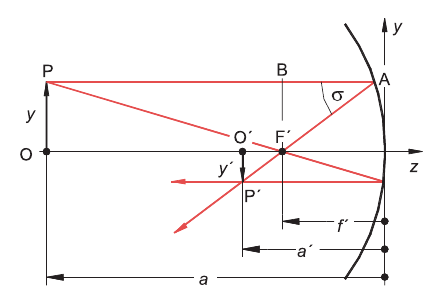
\includegraphics[width=50mm,keepaspectratio=true]{physik/png/optik1.png}
\end{boxleft}\begin{boxrightshaded}
\begin{align*}
\frac{1}{f'}&=\frac{1}{a}+\frac{1}{a'}\\
f'&=\frac{r}{2}\\
\beta'&=\frac{y'}{y}\\
\beta'&=-\frac{a'}{a}\\
a'&=\frac{af'}{a-f'}
\end{align*}
\end{boxrightshaded}

\subsection{Linse}

\begin{boxleft}\bla{Linse}
\des[\metre]{f'}{Brennpunkt}\\
\des[\metre]{a'}{Bildweite}\\
\des[\metre]{y'}{Bildgröße}\\
\des[\per\metre]{D'}{Brechkraft}\\
\des{n_L}{Brechzahl Linse}\\
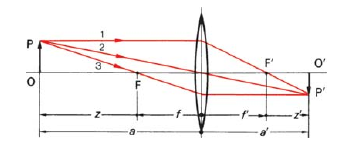
\includegraphics[width=50mm,keepaspectratio=true]{physik/png/optik2.png}
\end{boxleft}\begin{boxrightshaded}
\begin{align*}
\frac{1}{f'}&=\frac{1}{a'}-\frac{1}{a}\\
a'&=\frac{af'}{a+f'}\\
\beta'&=\frac{f'}{a+f'}\\
\beta'&=\frac{y'}{y}\\
D'&=\frac{1}{f'}=\left(n_L-1\right)\cdot\left(\frac{1}{r_1}-\frac{1}{r_2}\right)
\end{align*}
\end{boxrightshaded}


\begin{center}
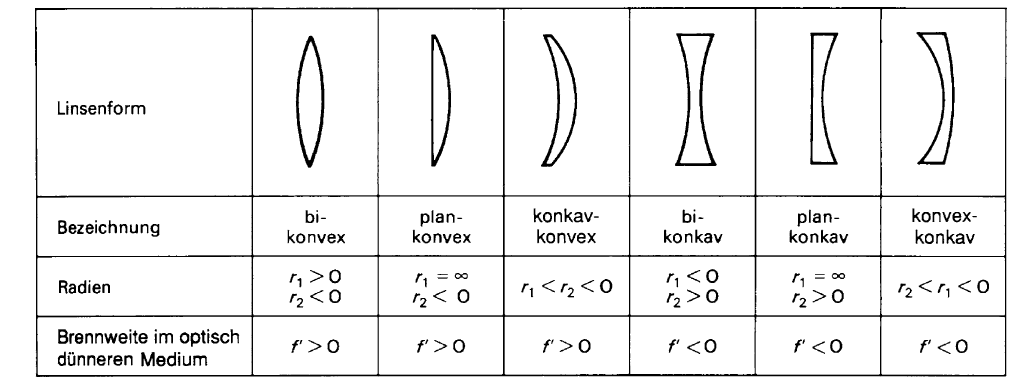
\includegraphics[width=150mm,keepaspectratio=true]{physik/png/optik3.png}
\end{center}

\subsection{LWL}

\begin{boxleft}\bla{Linse}
\des{A_{WL}}{numerische Aperatur}\\\\
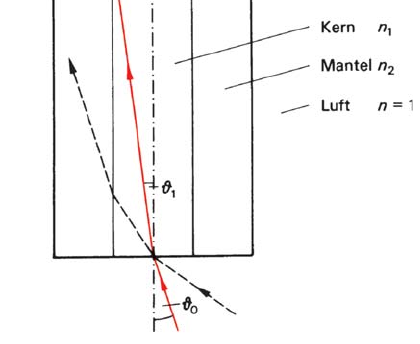
\includegraphics[width=50mm,keepaspectratio=true]{physik/png/optik4.png}
\end{boxleft}\begin{boxrightshaded}
\begin{align*}
n\sin\vartheta_0&=\sqrt{n_1^2-n_2^2}\\
A_{WL}&=\sqrt{n_1^2-n_2^2}
\end{align*}
\end{boxrightshaded}